\begin{document}
	The NMOS common source amplifer for this lab was constructed using 2N7000 NMOS transistors. The circuit essentially consists of two parts, the voltage amplifier stage and the current mirror. The generic circuit for the current driver is shown in Figure \ref{fig:currentgeneric}. 
	
	\begin{figure}[H]
		\centering
		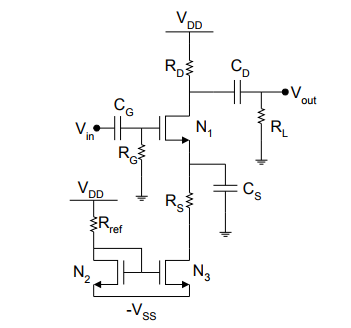
\includegraphics[width=.55\textwidth]{CircuitDevelopment/genericschem.png}
		\caption{Generic common source amplifier circuit \cite{b1}}
		\label{fig:currentgeneric}
	\end{figure}
	
	In order to understand the operation of the circuit, DC analysis of the circuit is required. At DC all the capacitors behave as shorts. It is known that the current through a MOSFET is seen in Equation \ref{eq:k}
	\begin{equation}\label{eq:k}
	I_D = k(V_{gs}-V_t)^2,
	\end{equation}
	
	Where k is the transconductance parameter, V$_{gs}$ is the gate-source voltage and V$_T$ is the threshold voltage. From the datasheet \cite{NMOS},  I$_D$ is 75 mA when V$_{gs}$ is 4.5 V. From Equation \ref{eq:k} k can be found to be 8.5 mA/V. Again using Equation \ref{eq:k}, the corresponding V$_{gs}$ for a bias current of 1 mA is found to be 1.85 V. 
	Upon finding the voltage drop over the NMOS, the source resistance can then be found by KCL across the amplifier NMOS. R$_{s}$ is found to be 8.3 k$\Omega$, R$_{ref}$ can found to be 22.2 k$\Omega$. AC analysis of the circuit is then required in order to find the drain resistance. Figure \ref{fig:smallsignalnmos} shows the equivalent small signal model for the NMOS.
	
	
	\begin{figure}[H]
		\centering
		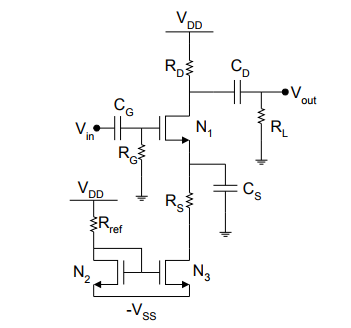
\includegraphics[width=.55\textwidth]{CircuitDevelopment/genericschem.png}
		\caption{Generic common source amplifier circuit \cite{b1}}
		\label{fig:currentgeneric}
	\end{figure}
	
	The transconductance of this circuit is defined as Equation \ref{eq:trancond}
	
	\begin{equation}\label{eq:trancond}
	g_m = \frac{2I_D}{V_{ov}},
	\end{equation}
	
	where V$_{ov}$ is the overdrive voltage. From this small signal transconductance is found to be 2.8 mA. The small signal r$_0$, defined as Equation \ref{eq:smallro}
	
	\begin{equation}\label{eq:smallro}
	
	r_o = \frac{1}{\lamda I_{DS}},
	
	\end{equation}
	
	where $\lambda$ is the body effect, and found from the datasheet \cite{NMOS} to be zero for the operating conditions. The open circuit gain can then be found by Equation \ref{eq:opengain} 
	
	\begin{equation}\label{eq:opengain}
	\frac{v_o}{v_{in}} = g_mR_o,
	\end{equation}
	
	where R$_o$ is the equivalent resistance of (R$_D$ || R$_L$). The load resistance is provided by the lab, but for this calculation can be assumed to nearly infinite, therefore R$_D$ is found to be around 2 k$\Omega$. The circuit was then simulated in NGSpice integrated with Matlab.
	
	
	A BJT, in contrast with the metal oxide semi-conducting field effect transistor (MOSFET), is capable of producing current by both types of Charge Carriers. This effectively allows the BJT to behave as a NPN or PNP transistor depending on the size of the input current. This also allows the BJT to use a smaller current signal to control a larger current. 
	
	The electrical properties of a BJT are paramount for this lab. The MCP6004 is only capable of outputting around 20mA of current. The IR LED in use, however, has a forward current of 100mA \cite{LEDDATA}. A much larger current has to generated in order for the LED to operate. Figure \ref{fig:ivsvled} shows the IV curve for the IR1503 LED.
	
	
	\begin{figure}[H]
		\centering
		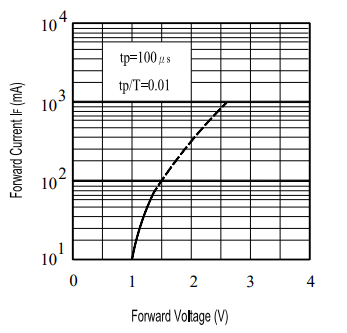
\includegraphics[width=0.4\linewidth]{CircuitDevelopment/IvsVled}
		\caption[Current vs voltage]{The IV characteristic of the IR1503 \cite{LEDDATA}}
		\label{fig:ivsvled}
	\end{figure}
	
	
	The MCP6004 is used to set the node voltage for R$_{sense}$. The op amp is assumed to be ideal, so $V_- = V_+$. In order to ensure that the LED is forward biased, the node voltage should be less than the sum of the voltage drops from $V_{supply}$ over the BJT and the diode \cite{b2}. The lab briefing \cite{b2} states to set $V_-$ less then 3V.
	
	In order to attain a suitable voltage, a voltage divider is placed at the input to the op amp. The source voltage is the output from the signal conditioner, and was found to be 5V. In order to be less than 3V, a 50/50 voltage divider was used in order to create an input of 2.5V. With this voltage, and the maximum forward current of 200mA, the value for R$_{sense}$ can solved using Ohm's Law. The final value for R$_{sense}$ is 12$\Omega$. The simulated circuit for current driver is seen in Figure \ref{fig:finalleddriverschem}.
	
	\begin{figure}[H]
		\centering
		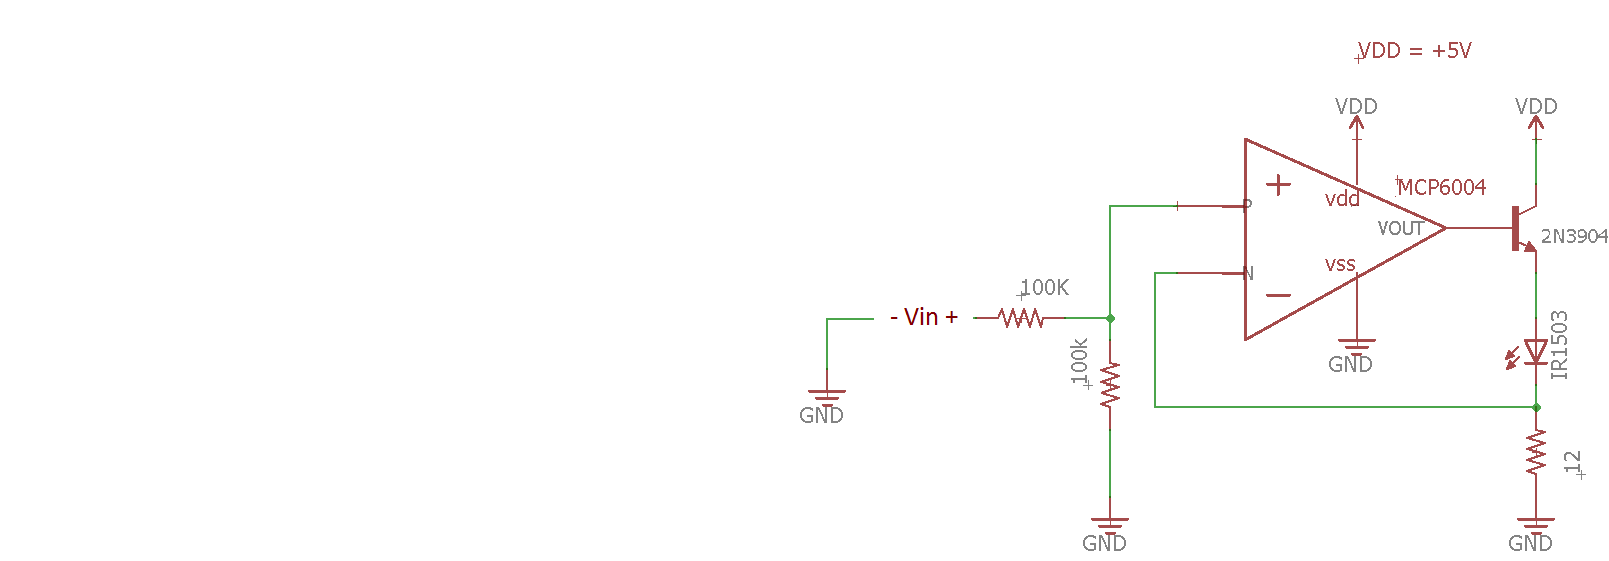
\includegraphics[width=0.6\linewidth]{CircuitDevelopment/FinalLEDdriverSChem}
		\caption[Simulated LED driver]{Simulated LED driver circuit}
		\label{fig:finalleddriverschem}
	\end{figure}
	
	The circuit required no changes from design to simulation. The current through the LED can be seen in Figure \ref{fig:simcurrentlab4}. The simulation was performed using a transient analysis in NGSpice integrated with Matlab.
	
	\begin{figure}[H]
		\centering
		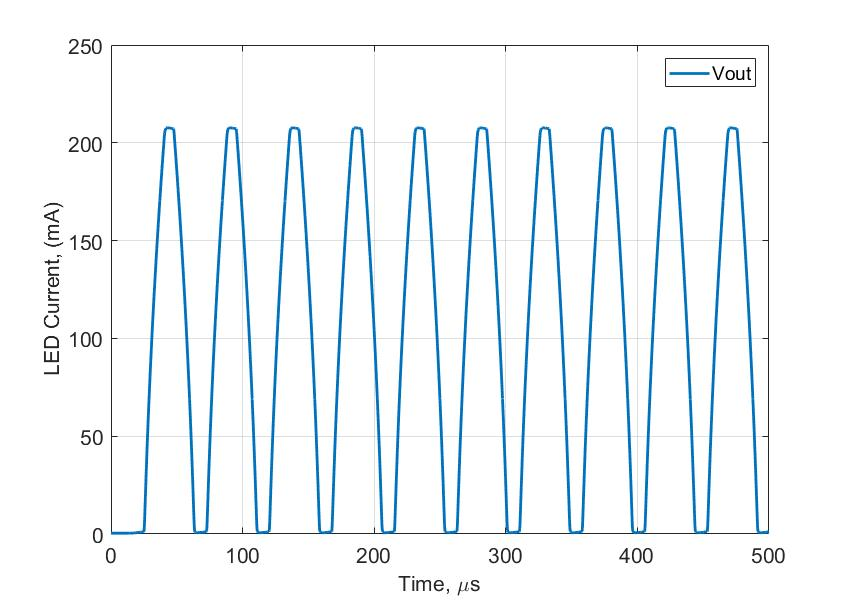
\includegraphics[width=0.60\linewidth]{CircuitDevelopment/sim_current_lab4}
		\caption[Simulated current]{Simulated current through the LED}
		\label{fig:simcurrentlab4}
	\end{figure}
	
	The current through the LED matched the calculated value of 200mA. The LED is in an operational state. The LED also operates with the correct frequency and duty-cycle from the signal conditioner.
	
	
	
\end{document}